\chapter{Технологическая часть}

В данной части обосновывается выбор средств реализации, приводится модульная структура разработанного программного обеспечения и описывается программная реализация ключевых алгоритмов визуализации, моделирования освещения и управления сценой.

\section{Выбор средств реализации}

Для разработки программного комплекса был выбран язык программирования \textbf{Python} версии 3.13 \cite{python_docs}. Выбор обусловлен следующими соображениями:
\begin{enumerate}
	\item Наличие библиотеки \textbf{NumPy} \cite{numpy_docs}, обеспечивающей векторизацию матричных операций. Поскольку рендеринг выполняется на центральном процессоре, использование низкоуровневых оптимизаций NumPy, реализованных на языке C, необходимо для повышения производительности вычислений.
	\item Кроссплатформенность, позволяющая исполнять приложение в операционных системах Windows, Linux и macOS без перекомпиляции исходного кода.
	\item Высокоуровневый синтаксис и динамическая типизация, упрощающие реализацию алгоритмической части.
\end{enumerate}

В качестве библиотеки графического интерфейса пользователя (GUI) используется \textbf{PyQt5} \cite{pyqt_docs}. Это набор привязок к фреймворку Qt, реализующий механизм сигналов и слотов \cite{qt_official}. Библиотека предоставляет набор элементов управления и средства работы с растровой графикой (классы \texttt{QImage} и \texttt{QPixmap}), используемые для вывода буфера кадра.

Разработка выполнялась в интегрированной среде \textbf{PyCharm}, содержащей инструменты отладки, рефакторинга и профилирования кода. Для сборки приложения в исполняемый файл применялся инструмент PyInstaller \cite{pyinstaller_docs}.

\section{Структура программы}

Программное обеспечение спроектировано с использованием модульной архитектуры, что упрощает поддержку и расширение функционала. Архитектура приложения и зависимости между модулями визуально представлены на диаграмме пакетов (рисунок \ref{fig:packages}).

\begin{figure}[H]
	\centering
	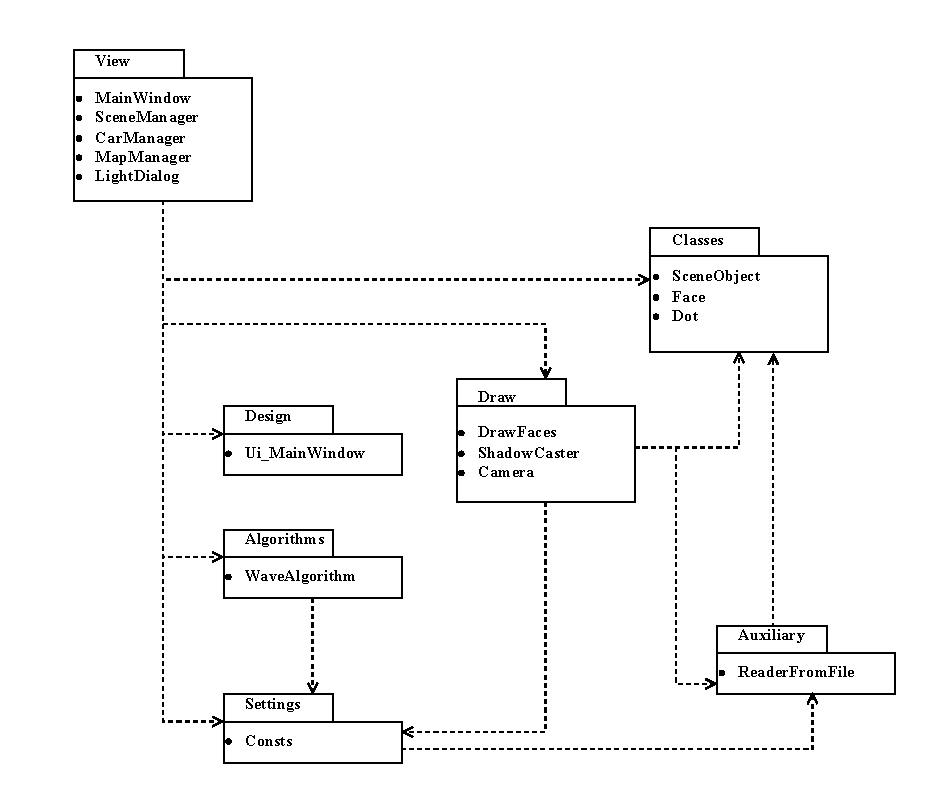
\includegraphics[width=0.9\textwidth]{img/algorithms/pacages.drawio}
	\caption{Диаграмма пакетов программного средства}
	\label{fig:packages}
\end{figure}

Основные модули и их назначение:

\begin{itemize}
	\item \textbf{main.py} — точка входа в приложение, инициализация главного окна.
	\item \textbf{settings/consts.py} — файл конфигурации, содержащий глобальные константы (разрешение рендеринга, параметры камеры, пути к ресурсам).
	\item \textbf{view/} — пакет, отвечающий за пользовательский интерфейс и логику взаимодействия:
	\begin{itemize}
		\item \texttt{main\_window.py} — класс главного окна, обработка событий таймера и ввода.
		\item \texttt{scene\_manager.py} — менеджер сцены, связывающий математическую модель с виджетом вывода.
		\item \texttt{light\_dialog.py} — диалоговое окно настройки источников света.
	\end{itemize}
	\item \textbf{draw/} — пакет, содержащий реализацию графического конвейера:
	\begin{itemize}
		\item \texttt{draw\_faces.py} — ядро рендеринга: алгоритмы растеризации, Z-буфер, расчет освещения.
		\item \texttt{shadows.py} — класс для генерации карт теней.
		\item \texttt{camera.py} — математическая модель камеры (матрицы вида и проекции).
	\end{itemize}
	\item \textbf{algorithms/} — пакет вспомогательных алгоритмов (поиск пути).
	\item \textbf{classes/} — описания структур данных (\texttt{SceneObject}, \texttt{Dot}, \texttt{Face}).
\end{itemize}

\section{Реализация алгоритмов визуализации}

Одной из наиболее трудоемких задач является реализация алгоритма построения теней (Shadow Mapping). Для этого был разработан класс \texttt{ShadowCaster}, который рассчитывает матрицы вида и проекции для источника света и формирует карту глубины.

В листинге \ref{lst:shadows} представлен код класса, отвечающего за создание матриц трансформации для источника света и рендеринг карты теней.

\captionsetup{singlelinecheck=false, justification=raggedright}
\begin{lstlisting}[language=Python, label=lst:shadows, caption=Реализация класса ShadowCaster (файл draw/shadows.py), basicstyle=\footnotesize\ttfamily, breaklines=true]
	import numpy as np
	from settings.consts import SHADOW_MAP_RES, LIGHT_ORTHO_SIZE
	
	class ShadowCaster:
	def __init__(self, light_config):
	raw_dir = np.array(light_config['dir'], dtype=float)
	norm = np.linalg.norm(raw_dir)
	if norm == 0:
	self.light_dir = np.array([0.0, 1.0, 0.0])
	else:
	self.light_dir = raw_dir / norm
	self.color = light_config['color']
	self.intensity = light_config['intensity']
	self.resolution = SHADOW_MAP_RES
	self.ortho_size = LIGHT_ORTHO_SIZE
	self.shadow_buffer = np.full((self.resolution, self.resolution), np.inf, dtype=np.float32)
	self.view_matrix = np.eye(4)
	self.proj_matrix = np.eye(4)
	self.vp_matrix = np.eye(4)
	self._calculate_matrices()
	
	def _calculate_matrices(self):
	target = np.array([0.0, 0.0, 0.0])
	position = target + self.light_dir * 50.0
	up = np.array([0.0, 1.0, 0.0])
	if abs(np.dot(self.light_dir, up)) > 0.95:
	up = np.array([0.0, 0.0, 1.0])
	forward = target - position
	forward /= np.linalg.norm(forward)
	right = np.cross(forward, up)
	right /= np.linalg.norm(right)
	real_up = np.cross(right, forward)
	self.view_matrix = np.eye(4)
	self.view_matrix[0, :3] = right
	self.view_matrix[1, :3] = real_up
	self.view_matrix[2, :3] = -forward
	self.view_matrix[:3, 3] = -np.array([
	np.dot(right, position),
	np.dot(real_up, position),
	np.dot(-forward, position)
	])
	r = self.ortho_size
	l = -self.ortho_size
	t = self.ortho_size
	b = -self.ortho_size
	n = 1.0
	f = 100.0
	self.proj_matrix = np.array([
	[2 / (r - l), 0, 0, -(r + l) / (r - l)],
	[0, 2 / (t - b), 0, -(t + b) / (t - b)],
	[0, 0, -2 / (f - n), -(f + n) / (f - n)],
	[0, 0, 0, 1]
	])
	self.vp_matrix = self.proj_matrix @ self.view_matrix
	
	def transform_poly_to_light_space(self, vertices):
	res_coords = []
	for v in vertices:
	vec = np.array([v.x, v.y, v.z, 1.0])
	clip = self.vp_matrix @ vec
	w = clip[3] if clip[3] != 0 else 1.0
	ndc_x = clip[0] / w
	ndc_y = clip[1] / w
	ndc_z = clip[2] / w
	screen_x = (ndc_x + 1) * 0.5 * (self.resolution - 1)
	screen_y = (1 - ndc_y) * 0.5 * (self.resolution - 1)
	depth = ndc_z * 0.5 + 0.5
	res_coords.append((screen_x, screen_y, depth))
	return res_coords
	
	def render_shadow_map(self, faces):
	self.shadow_buffer.fill(np.inf)
	for face in faces:
	coords = self.transform_poly_to_light_space(face.vertices)
	xs = [c[0] for c in coords]
	ys = [c[1] for c in coords]
	if max(xs) < 0 or min(xs) >= self.resolution or max(ys) < 0 or min(ys) >= self.resolution:
	continue
	n_verts = len(coords)
	min_y = max(0, int(np.floor(min(ys))))
	max_y = min(self.resolution - 1, int(np.ceil(max(ys))))
	for y in range(min_y, max_y + 1):
	intersections = []
	for i in range(n_verts):
	v1 = coords[i]
	v2 = coords[(i + 1) % n_verts]
	if (v1[1] <= y < v2[1]) or (v2[1] <= y < v1[1]):
	if abs(v2[1] - v1[1]) < 1e-9: continue
	t = (y - v1[1]) / (v2[1] - v1[1])
	x_int = v1[0] + t * (v2[0] - v1[0])
	z_int = v1[2] + t * (v2[2] - v1[2])
	intersections.append((x_int, z_int))
	intersections.sort(key=lambda p: p[0])
	for k in range(0, len(intersections) - 1, 2):
	left = intersections[k]
	right = intersections[k + 1]
	x_start = max(0, int(np.ceil(left[0])))
	x_end = min(self.resolution - 1, int(np.ceil(right[0])))
	if x_end < x_start: continue
	width = right[0] - left[0]
	if width < 1e-9: continue
	xx = np.arange(x_start, x_end + 1)
	t_span = (xx - left[0]) / width
	z_vals = left[1] + t_span * (right[1] - left[1])
	current_depths = self.shadow_buffer[y, x_start:x_end + 1]
	mask = z_vals < current_depths
	self.shadow_buffer[y, x_start:x_end + 1][mask] = z_vals[mask]
\end{lstlisting}

\section{Реализация алгоритма отрисовки сцены}

Основной алгоритм визуализации реализован в модуле \texttt{draw\_faces.py}. Он выполняет сбор геометрических данных, расчет освещения и наложение текстур.

В листинге \ref{lst:rasterize} приведена функция, которая реализует построчное сканирование полигона (Scanline) с использованием Z-буфера и проверкой карты теней для каждого пикселя. Для ускорения работы внутренние циклы векторизованы с использованием массивов NumPy.

\captionsetup{singlelinecheck=false, justification=raggedright}
\begin{lstlisting}[language=Python, label=lst:rasterize, caption=Реализация алгоритма растеризации грани (файл draw/draw\_faces.py), basicstyle=\footnotesize\ttfamily, breaklines=true]
	def rasterize_face_with_shadows(face, zbuffer, img_array, cam, shadow_casters, current_scale):
	if len(face.vertices) < 3: return
	screen_coords = []
	for v in face.vertices:
	sx, sy, sz = project_vertex(v, cam, current_scale)
	if not (np.isfinite(sx) and np.isfinite(sy) and np.isfinite(sz)): return
	screen_coords.append((sx, sy, sz))
	xs = np.array([p[0] for p in screen_coords])
	ys = np.array([p[1] for p in screen_coords])
	min_x, max_x = int(np.floor(np.min(xs))), int(np.ceil(np.max(xs)))
	min_y, max_y = int(np.floor(np.min(ys))), int(np.ceil(np.max(ys)))
	if max_x < 0 or min_x >= WIDTH_CANVAS or max_y < 0 or min_y >= HEIGHT_CANVAS: return
	min_y = max(0, min_y)
	max_y = min(HEIGHT_CANVAS - 1, max_y)
	color_key = tuple(face.color)
	is_textured = (face.uv is not None and color_key in TEXTURES and TEXTURES[color_key] is not None)
	texture_data = TEXTURES[color_key] if is_textured else None
	uv_coords = face.uv if is_textured else None
	texture_repeat = TEXTURE_REPEAT_MAP.get(color_key, DEFAULT_TEXTURE_REPEAT)
	normal = calculate_face_normal(face.vertices)
	casters_data = []
	for caster in shadow_casters:
	light_dir = caster.light_dir
	diff = abs(np.dot(normal, light_dir))
	s_coords = caster.transform_poly_to_light_space(face.vertices)
	casters_data.append({'caster': caster, 'diffuse': diff, 's_coords': s_coords})
	n_verts = len(face.vertices)
	for y in range(min_y, max_y + 1):
	intersections = []
	for i in range(n_verts):
	v1 = screen_coords[i]
	v2 = screen_coords[(i + 1) % n_verts]
	y1, y2 = v1[1], v2[1]
	if (y1 <= y < y2) or (y2 <= y < y1):
	if abs(y2 - y1) < 1e-9: continue
	t = (y - y1) / (y2 - y1)
	x_int = v1[0] + t * (v2[0] - v1[0])
	z_int = v1[2] + t * (v2[2] - v1[2])
	sc_list = []
	for c_data in casters_data:
	s_poly = c_data['s_coords']
	s1 = s_poly[i]
	s2 = s_poly[(i + 1) % n_verts]
	s_int = (s1[0] + t * (s2[0] - s1[0]), s1[1] + t * (s2[1] - s1[1]), s1[2] + t * (s2[2] - s1[2]))
	sc_list.append(s_int)
	uvc = (0,0)
	if is_textured:
	u1, v1_uv = uv_coords[i]
	u2, v2_uv = uv_coords[(i + 1) % n_verts]
	uvc = (u1 + t*(u2-u1), v1_uv + t*(v2_uv-v1_uv))
	intersections.append((x_int, z_int, sc_list, uvc))
	intersections.sort(key=lambda p: p[0])
	for k in range(0, len(intersections) - 1, 2):
	left = intersections[k]
	right = intersections[k+1]
	x_start = int(np.ceil(left[0]))
	x_end = int(np.ceil(right[0]))
	x_start = max(0, min(x_start, WIDTH_CANVAS - 1))
	x_end = max(0, min(x_end, WIDTH_CANVAS - 1))
	if x_end <= x_start: continue
	span_width = right[0] - left[0]
	if span_width < 1e-9: continue
	pixel_x = np.arange(x_start, x_end + 1, dtype=np.float32)
	t_span = (pixel_x - left[0]) / span_width
	z_left, z_right = left[1], right[1]
	z_vals = z_left + t_span * (z_right - z_left)
	current_z = zbuffer[y, x_start:x_end+1]
	visible_mask = z_vals < current_z
	if not np.any(visible_mask): continue
	indices = np.where(visible_mask)[0]
	full_indices = x_start + indices
	zbuffer[y, full_indices] = z_vals[indices]
	t_vis = t_span[indices]
	final_intensity = np.full(len(indices), AMBIENT_INTENSITY, dtype=np.float32)
	for idx, c_data in enumerate(casters_data):
	caster = c_data['caster']
	diffuse = c_data['diffuse']
	sl = np.array(left[2][idx])
	sr = np.array(right[2][idx])
	s_vis = sl + t_vis[:, np.newaxis] * (sr - sl)
	map_x = s_vis[:, 0].astype(np.int32)
	map_y = s_vis[:, 1].astype(np.int32)
	v_d = s_vis[:, 2]
	in_map = (map_x >= 0) & (map_x < caster.resolution) & (map_y >= 0) & (map_y < caster.resolution) & (v_d >= 0) & (v_d <= 1.0)
	light_contrib = np.zeros(len(indices), dtype=np.float32)
	if np.any(in_map):
	valid_d = v_d[in_map]
	closest = caster.shadow_buffer[map_y[in_map], map_x[in_map]]
	lit_mask = valid_d <= (closest + SHADOW_BIAS)
	light_contrib[in_map] += np.where(lit_mask, 1.0, 0.0) * (diffuse * caster.intensity)
	final_intensity += light_contrib
	final_intensity = np.clip(final_intensity, 0.0, 1.0)
	if is_textured and texture_data:
	uv_l = np.array(left[3])
	uv_r = np.array(right[3])
	uv_vis = uv_l + t_vis[:, np.newaxis] * (uv_r - uv_l)
	tex_w = texture_data['width'] - 1
	tex_h = texture_data['height'] - 1
	tex_img = texture_data['array']
	u_fin = (uv_vis[:, 0] * texture_repeat) % 1.0
	v_fin = (uv_vis[:, 1] * texture_repeat) % 1.0
	tx = (u_fin * tex_w).astype(np.int32)
	ty = (v_fin * tex_h).astype(np.int32)
	base_colors = tex_img[ty, tx].astype(np.float32)
	else:
	base_colors = np.array(face.color, dtype=np.float32)
	res_colors = base_colors * final_intensity[:, np.newaxis]
	img_array[y, full_indices, 0] = res_colors[:, 2]
	img_array[y, full_indices, 1] = res_colors[:, 1]
	img_array[y, full_indices, 2] = res_colors[:, 0]
\end{lstlisting}

В листинге \ref{lst:main_draw} приведена функция, объединяющая все этапы конвейера: инициализацию буферов, генерацию теней для всех источников и финальную отрисовку.

\captionsetup{singlelinecheck=false, justification=raggedright}
\begin{lstlisting}[language=Python, label=lst:main_draw, caption=Управляющая функция отрисовки сцены (файл draw/draw\_faces.py), basicstyle=\footnotesize\ttfamily, breaklines=true]
	def draw_scene_with_objects(label_field, faces, cam, current_scale, objects=[]):
	all_faces = []
	all_faces.extend(faces)
	for obj in objects:
	all_faces.extend(obj.transformed_faces())
	auto_uv_unwrap(all_faces)
	casters = init_lighting_system()
	if casters:
	for caster in casters:
	caster.render_shadow_map(all_faces)
	img_array = np.zeros((HEIGHT_CANVAS, WIDTH_CANVAS, 4), dtype=np.uint8)
	img_array[:, :, 3] = 255
	zbuffer = np.full((HEIGHT_CANVAS, WIDTH_CANVAS), np.inf, dtype=np.float32)
	for face in all_faces:
	rasterize_face_with_shadows(face, zbuffer, img_array, cam, casters, current_scale)
	height, width, channels = img_array.shape
	bytes_per_line = channels * width
	image = QImage(img_array.data, width, height, bytes_per_line, QImage.Format_RGB32).copy()
	label_field.setPixmap(QPixmap.fromImage(image))
\end{lstlisting}

\section{Управление сценой и взаимодействие с пользователем}

Класс \texttt{SceneManager} отвечает за обработку пользовательского ввода (клавиатура, мышь) и обновление параметров сцены, таких как положение камеры и масштаб отображения. Его реализация приведена в листинге \ref{lst:scene_manager}.

\captionsetup{singlelinecheck=false, justification=raggedright}
\begin{lstlisting}[language=Python, label=lst:scene_manager, caption=Менеджер сцены (файл view/scene\_manager.py), basicstyle=\footnotesize\ttfamily, breaklines=true]
	class SceneManager:
	def __init__(self, label_field):
	self.label_field = label_field
	self.dots, self.edges, self.faces = [], [], []
	self.objects = []
	self.pressed_keys = set()
	self.current_scale = SCALE
	self.camera = Camera(
	position=DEFAULT_CAMERA_POSITION,
	target=DEFAULT_CAMERA_LOOK_AT,
	up=DEFAULT_CAMERA_UP,
	fov=DEFAULT_CAMERA_FOV
	)
	self.init_canvas()
	
	def init_canvas(self):
	self.canvas = QImage(WIDTH_CANVAS, HEIGHT_CANVAS, QImage.Format_RGB32)
	self.canvas.fill(Qt.black)
	self.label_field.setPixmap(QPixmap.fromImage(self.canvas))
	
	def load_scene_data(self):
	reader_from_file(filename=FILENAME_MAP, dots=self.dots, edges=self.edges, faces=self.faces)
	
	def add_object(self, obj):
	self.objects.append(obj)
	
	def update_scene(self):
	if Qt.Key_Q in self.pressed_keys:
	self.current_scale += ZOOM_SPEED
	if Qt.Key_E in self.pressed_keys:
	self.current_scale -= ZOOM_SPEED
	self.current_scale = max(SCALE, min(self.current_scale, MAX_SCALE))
	update_action(self.label_field, self.faces, self.pressed_keys, self.camera, self.current_scale, objects=self.objects)
	
	def key_press_event(self, event):
	if event.isAutoRepeat(): return
	self.pressed_keys.add(event.key())
	
	def key_release_event(self, event):
	if event.isAutoRepeat(): return
	if event.key() in self.pressed_keys:
	self.pressed_keys.remove(event.key())
\end{lstlisting}

\section{Описание интерфейса программы}

Главное окно программы (рисунок \ref{fig:screenshot_main}) разделено на две функциональные области. Слева находится область визуализации, занимающая основную часть экрана. Здесь отображается трехмерная сцена города, автомобиль и элементы интерфейса, такие как счетчик кадров в секунду.

\begin{figure}[H]
	\centering
	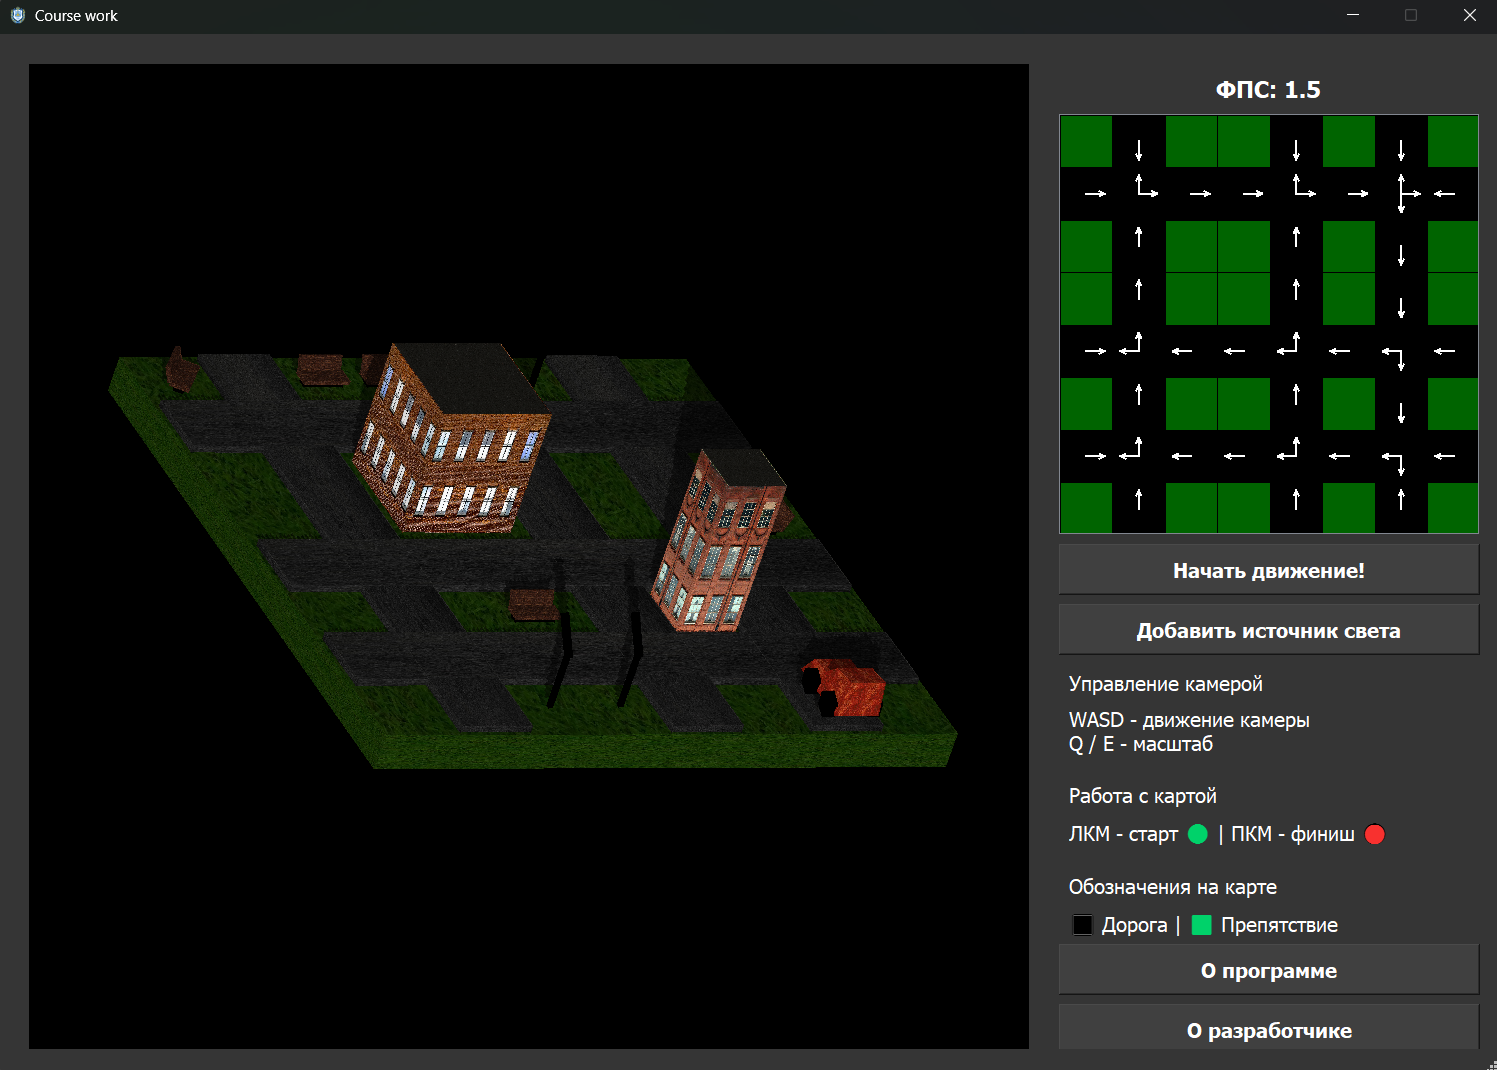
\includegraphics[width=0.9\textwidth]{img/screenshot_main}
	\caption{Главное окно программы}
	\label{fig:screenshot_main}
\end{figure}

Справа расположена панель управления. В её верхней части находится интерактивная карта (рисунок \ref{fig:screenshot_map}), которая визуализирует топологию дорожной сети. С помощью карты пользователь задает начальную (зеленый маркер) и конечную (красный маркер) точки маршрута, используя левую и правую кнопки мыши соответственно. Также на карте отображаются разрешенные направления движения в виде стрелок.

\begin{figure}[H]
	\centering
	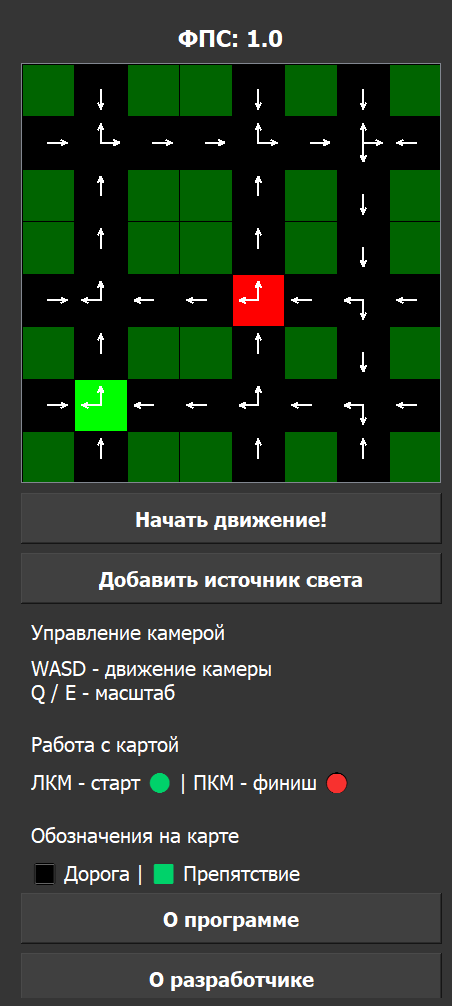
\includegraphics[width=0.5\textwidth]{img/screenshot_map}
	\caption{Интерфейс выбора маршрута (мини-карта)}
	\label{fig:screenshot_map}
\end{figure}

Для управления условиями освещения предусмотрено модальное окно (рисунок \ref{fig:screenshot_light}), вызываемое по кнопке «Добавить источник света». Оно позволяет задать вектор направления света и его интенсивность.

\begin{figure}[H]
	\centering
	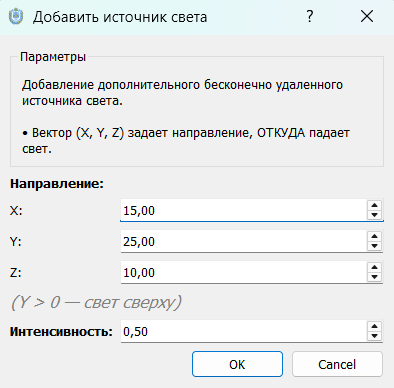
\includegraphics[width=0.6\textwidth]{img/screenshot_light}
	\caption{Диалоговое окно настройки освещения}
	\label{fig:screenshot_light}
\end{figure}

\section{Выводы по технологической части}

В данном разделе был обоснован выбор языка Python и библиотеки PyQt5 для реализации программного комплекса. Подробно описана структура проекта и реализация ключевых алгоритмов визуализации, включая построчное сканирование, Z-буфер и Shadow Mapping. Приведены листинги кода основных модулей. Разработанное программное обеспечение обладает модульной структурой, что облегчает его дальнейшее сопровождение и развитие.